%\documentclass[11pt,a4paper]{article}
\documentclass[11pt
  , a4paper
  , article
  , oneside
%  , twoside
%  , draft
]{memoir}

\usepackage{control}
\usepackage[numbers]{natbib}


\begin{document}

\newcommand{\technumber}{
  RAON Control-Document Series\\
  Revision : v0.1,   Release : a fixed date}
\title{\textbf{Your Technical Documentation \\Title}}



\author{your name\thanks{@ibs.re.kr} \\
  Control Team \\
  Rare Isotope Science Project\\
  Institute for Basic Science\\
  Daejeon, South Korea
}

\date{\today}

\renewcommand{\maketitlehooka}{\begin{flushright}\textsf{\technumber}\end{flushright}}
%\renewcommand{\maketitlehookb}{\centering\textsf{\subtitle}}
%\renewcommand{\maketitlehookc}{C}
%\renewcommand{\maketitlehookd}{D}

\maketitle

\begin{abstract}
Abstract and citations.... \citep{FAI}. 
\end{abstract}



\chapter{chapter}

\section{section}
\subsection{subsection}

\section{Figure and Itemize}
 Figure~\ref{fig:vmplayer_network} shows the vmplayer screen-shot of the MAC address for a virtual PC.

For the installation examples, two MAC addresses and the hostnames are used as follows :
\begin{itemize}
\item demohost  : \texttt{E8:03:9A:63:83:81}
\item gnomehost : \texttt{00:50:56:39:D9:1E}
\end{itemize}
\begin{figure}[!htb]
  \centering
  \includegraphics[width=0.96\textwidth]{./images/vmplayer_network.eps}
  \caption{
            MAC address setup for a virtual PC by using vmplayer.
          }
  \label{fig:vmplayer_network}   
\end{figure}



\clearpage

\chapter{Item and verbatim}

\begin{itemize}
  \item \texttt{/etc/fai}
    {\scriptsize
     \begin{verbatim}
      root@faiserver:/etc/fai# tree
      .
      ├── apt
      │   └── sources.list
      ├── fai.conf
      ├── grub.cfg
      ├── live.conf
      ├── NFSROOT
      └── nfsroot.conf
     \end{verbatim}
     }
  \item \texttt{/srv/fai}
    {\scriptsize
     \begin{verbatim}
      root@faiserver:/srv# tree -d -L 3
      .
      ├── fai
      │   ├── config
      │   │   ├── basefiles
      │   │   ├── class
      │   │   ├── debconf
      │   │   ├── disk_config
      │   │   ├── files
      │       ├── selinux
      │       ├── srv
      │       ├── sys
      │       ├── tmp
      │       ├── usr
      │       └── var
      └── tftp
            └── fai
                  └── pxelinux.cfg
  \end{verbatim}
  }
\end{itemize}

\subsection{lstlisting with termstyle}

termstyle is defined in control.sty

\begin{lstlisting}[style=termstyle]
root@faiserver:/etc/fai/apt# emacs /etc/fai/nfsroot.conf 

  # Configuration space
  FAI_CONFIGDIR=/srv/fai/config
\end{lstlisting}


\subsection{lstlisting with ternstylenumber and caption, label, reference  ... }

Line number is referred by \ref{firmware-linux-nonfree} and Listing can be done via Listing~\ref{list:nfsroot-file}. 

\begin{lstlisting}[style=termstylenumber, caption={Editing \texttt{/etc/fai/NFSROOT}}, label={list:nfsroot-file}]
   firmware-bnx2 firmware-bnx2x firmware-realtek
   firmware-linux-nonfree        (*@\label{firmware-linux-nonfree}@*) 

    # packages for Ubuntu natty/oneiric/precise:
   # linux-image-generic live-boot
\end{lstlisting}



\section{Figures}
Figure~\ref{fig:gnomehost} shows six images in one figure enviroment.

\begin{figure}[!htb]
  \centering
 
  \subbottom[F12 lets us to boot this host]
	    {
	      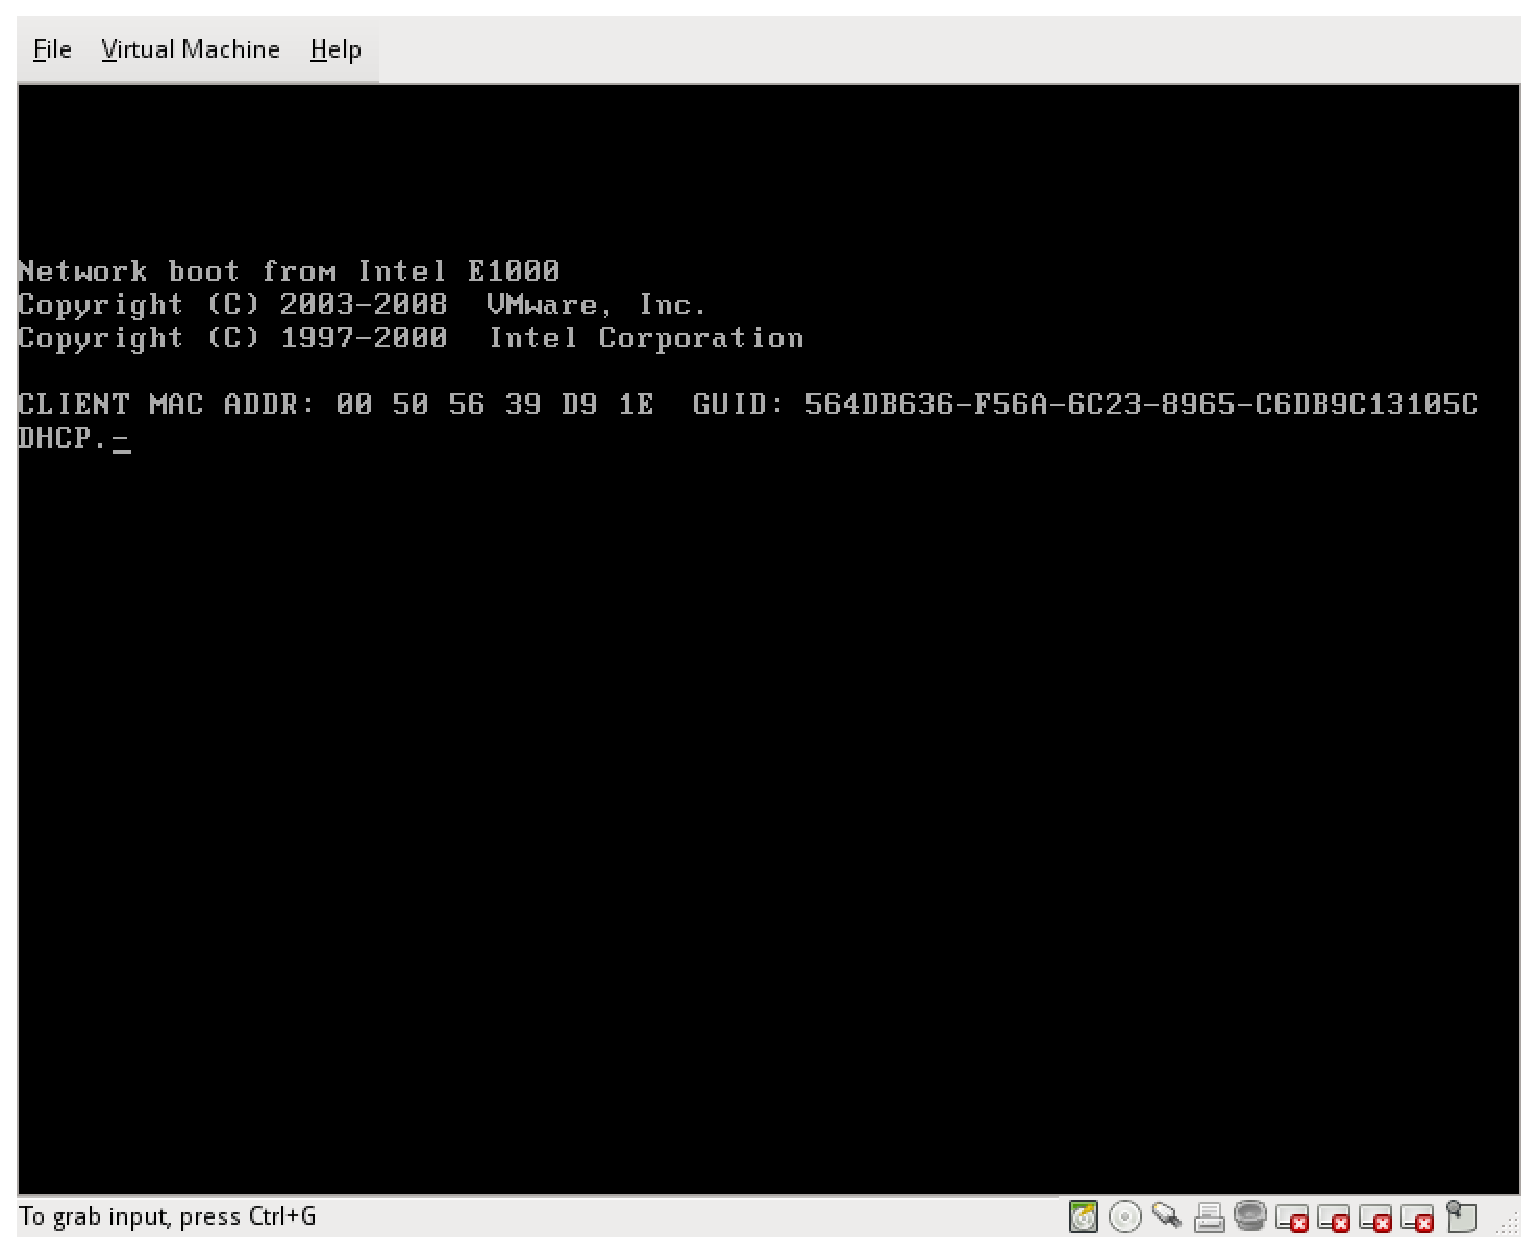
\includegraphics[width=0.45\textwidth]{./images/f-0.eps}
	      \label{fig:f-0}
	    }
            \hfill
  \subbottom[Booting .... ]
	    {
	      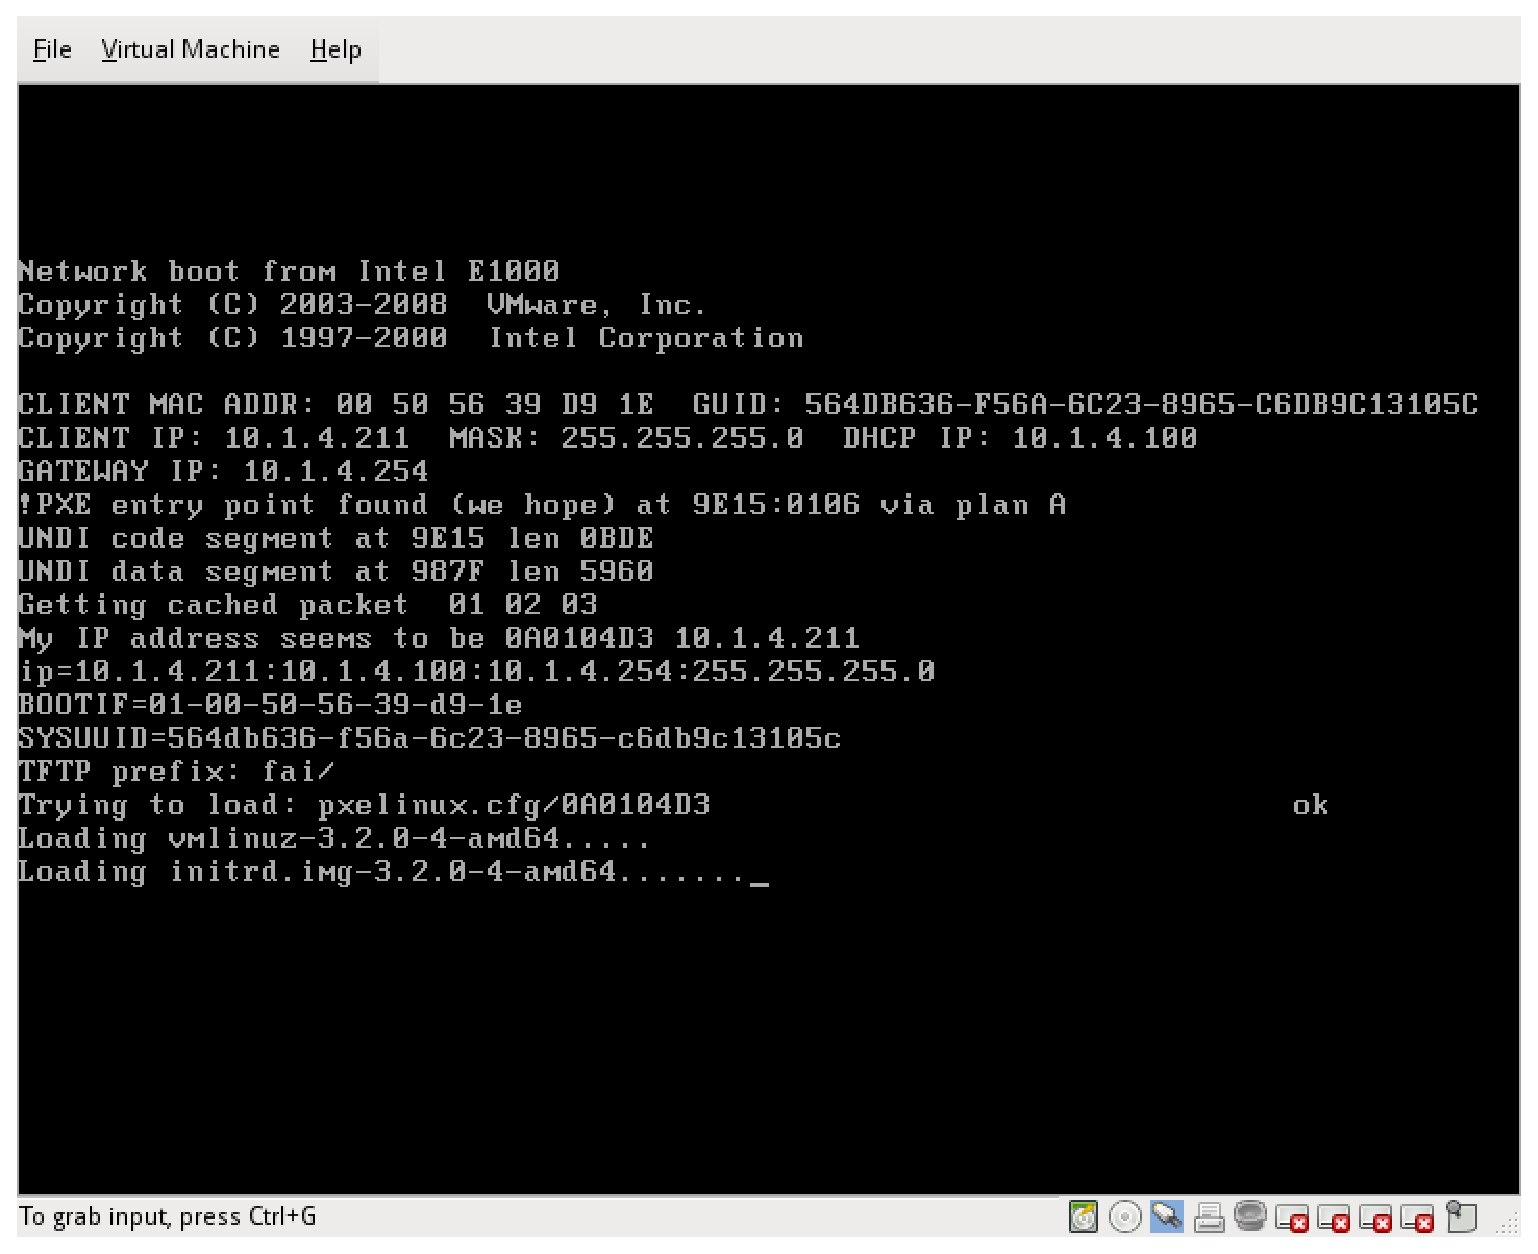
\includegraphics[width=0.45\textwidth]{./images/f-1.eps}
	      \label{fig:f-1}
	    }
            \subbottom[Clearly see the FAI Screen]
	    {
	      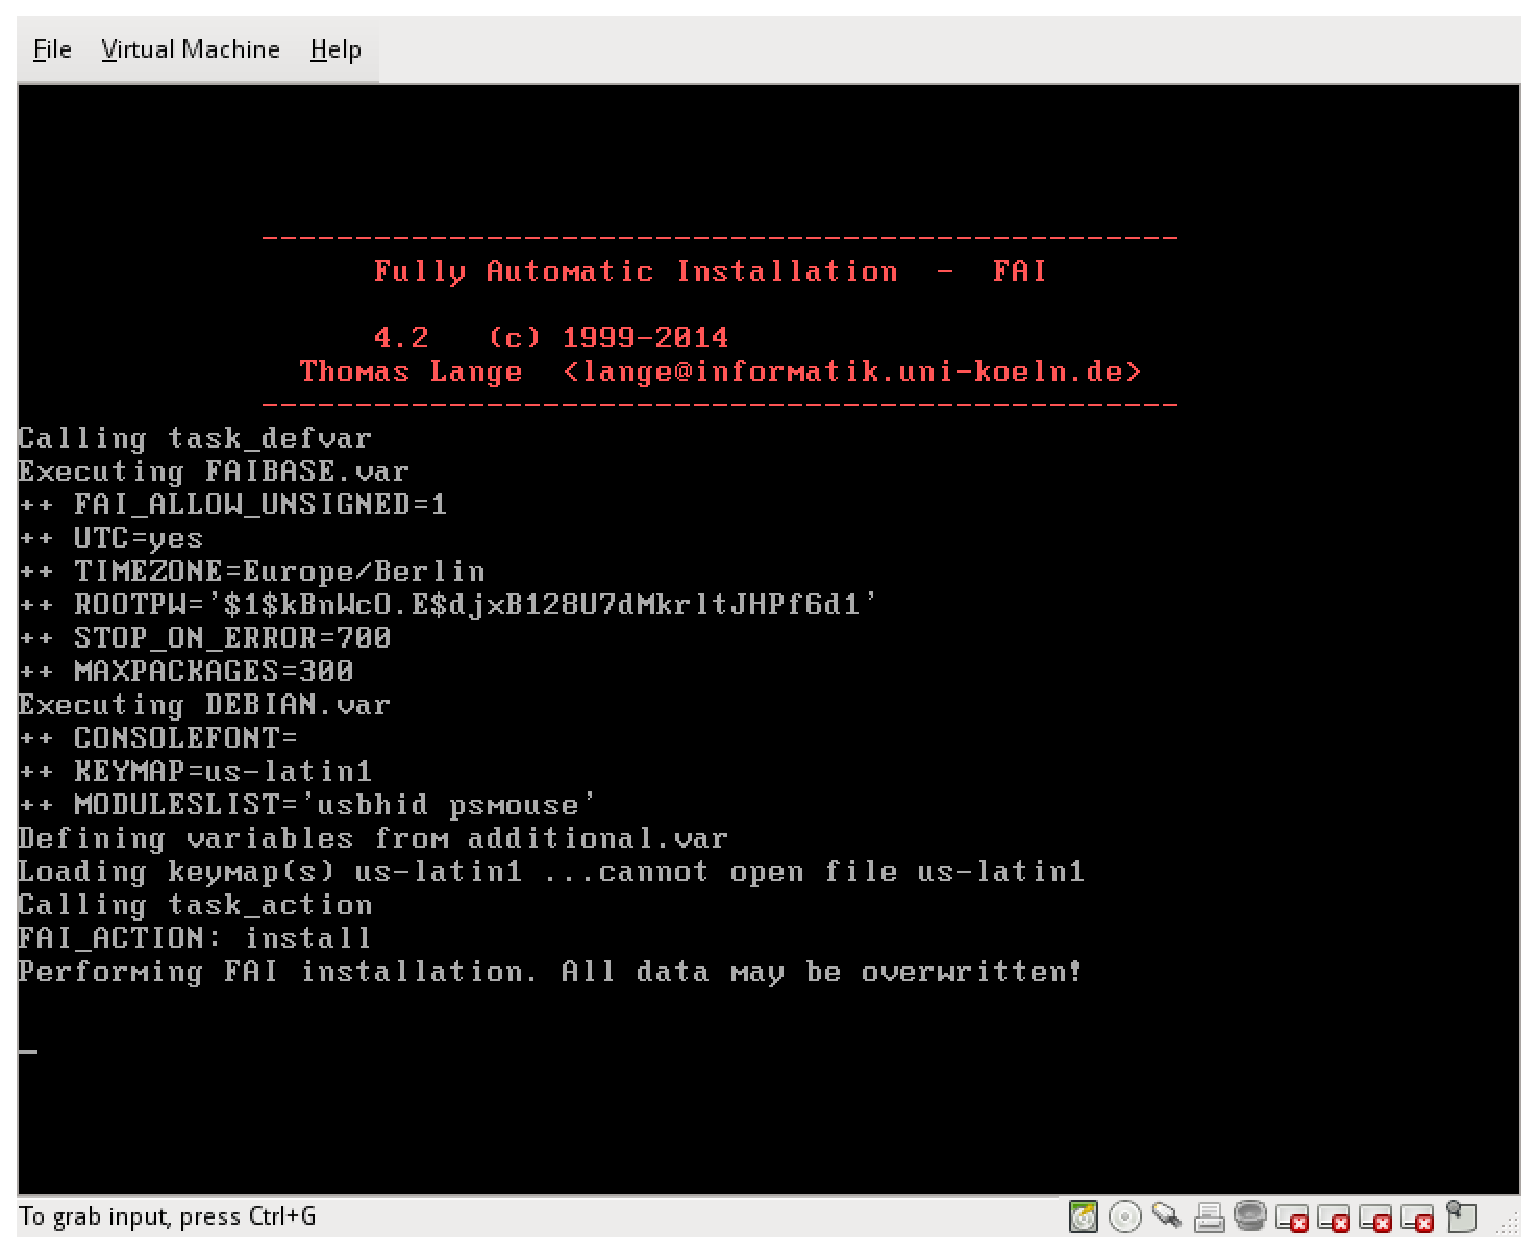
\includegraphics[width=0.45\textwidth]{./images/f-2.eps}
	      \label{fig:f-2}
	    }
            \hfill
  \subbottom[After reboot, the grub screen is shown]
	    {
	      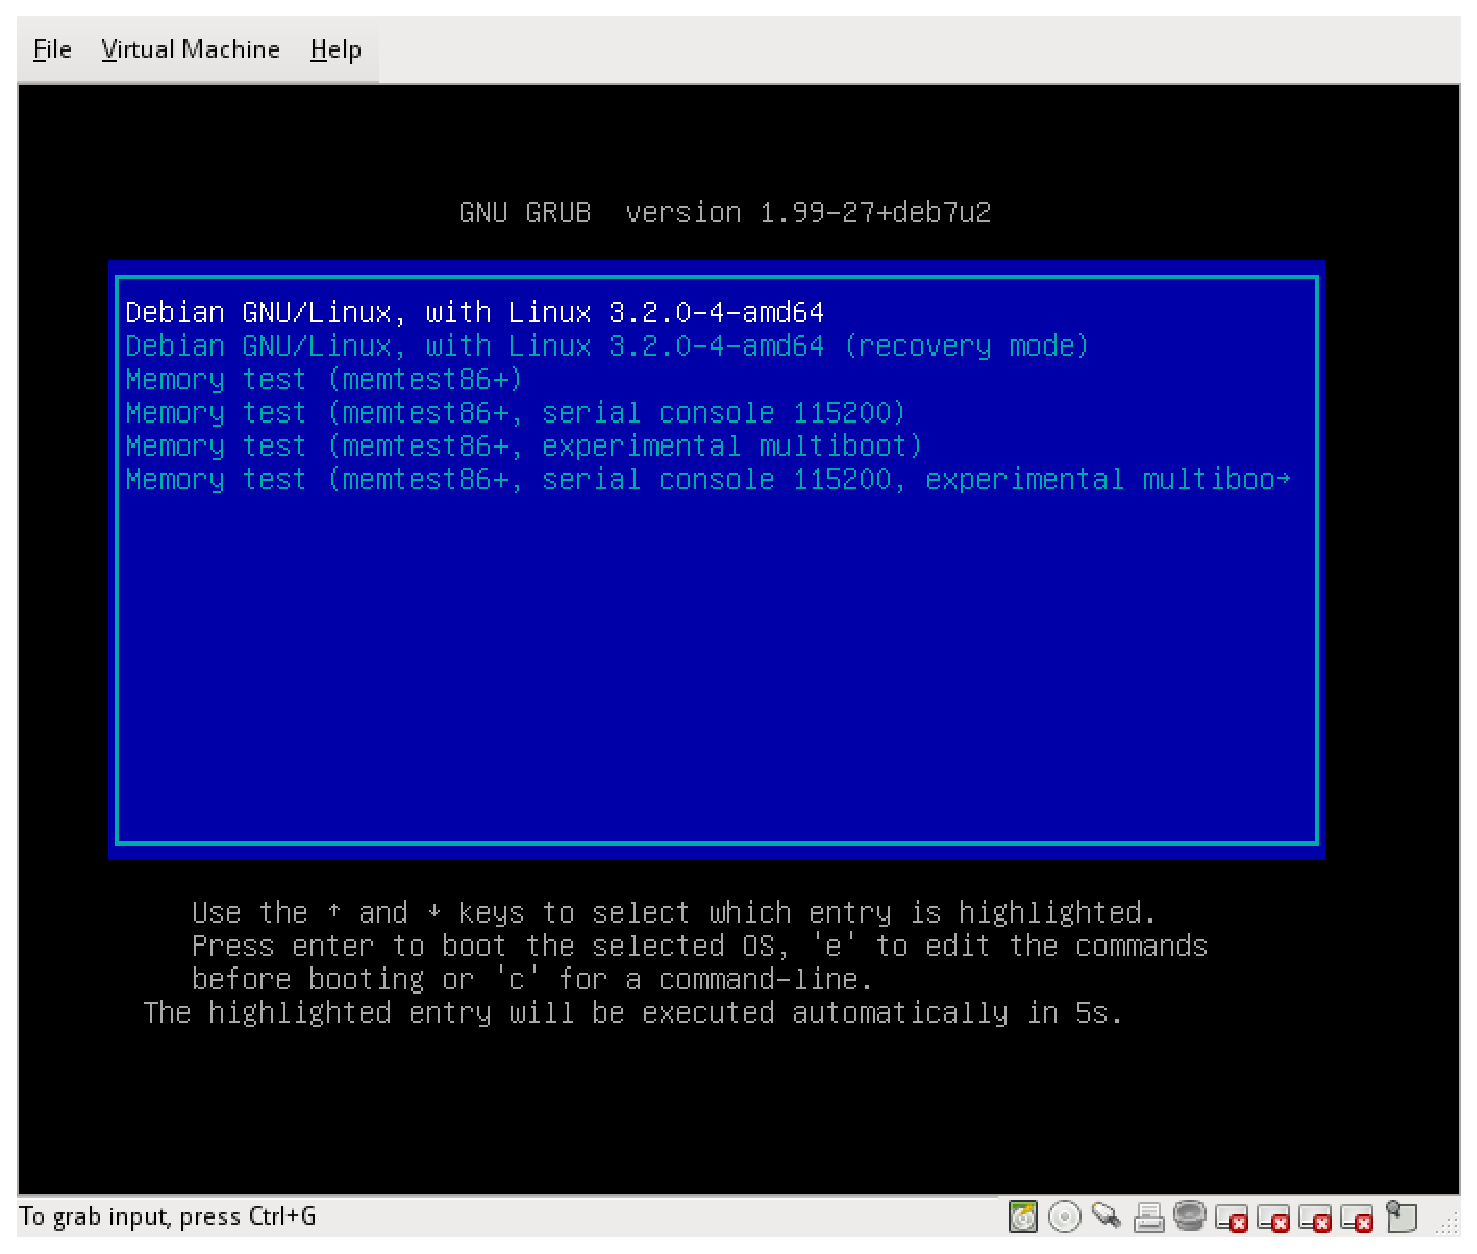
\includegraphics[width=0.45\textwidth]{./images/f-3.eps}
	      \label{fig:f-3}
	    }
            \subbottom[GNOME login screen]
	    {
	      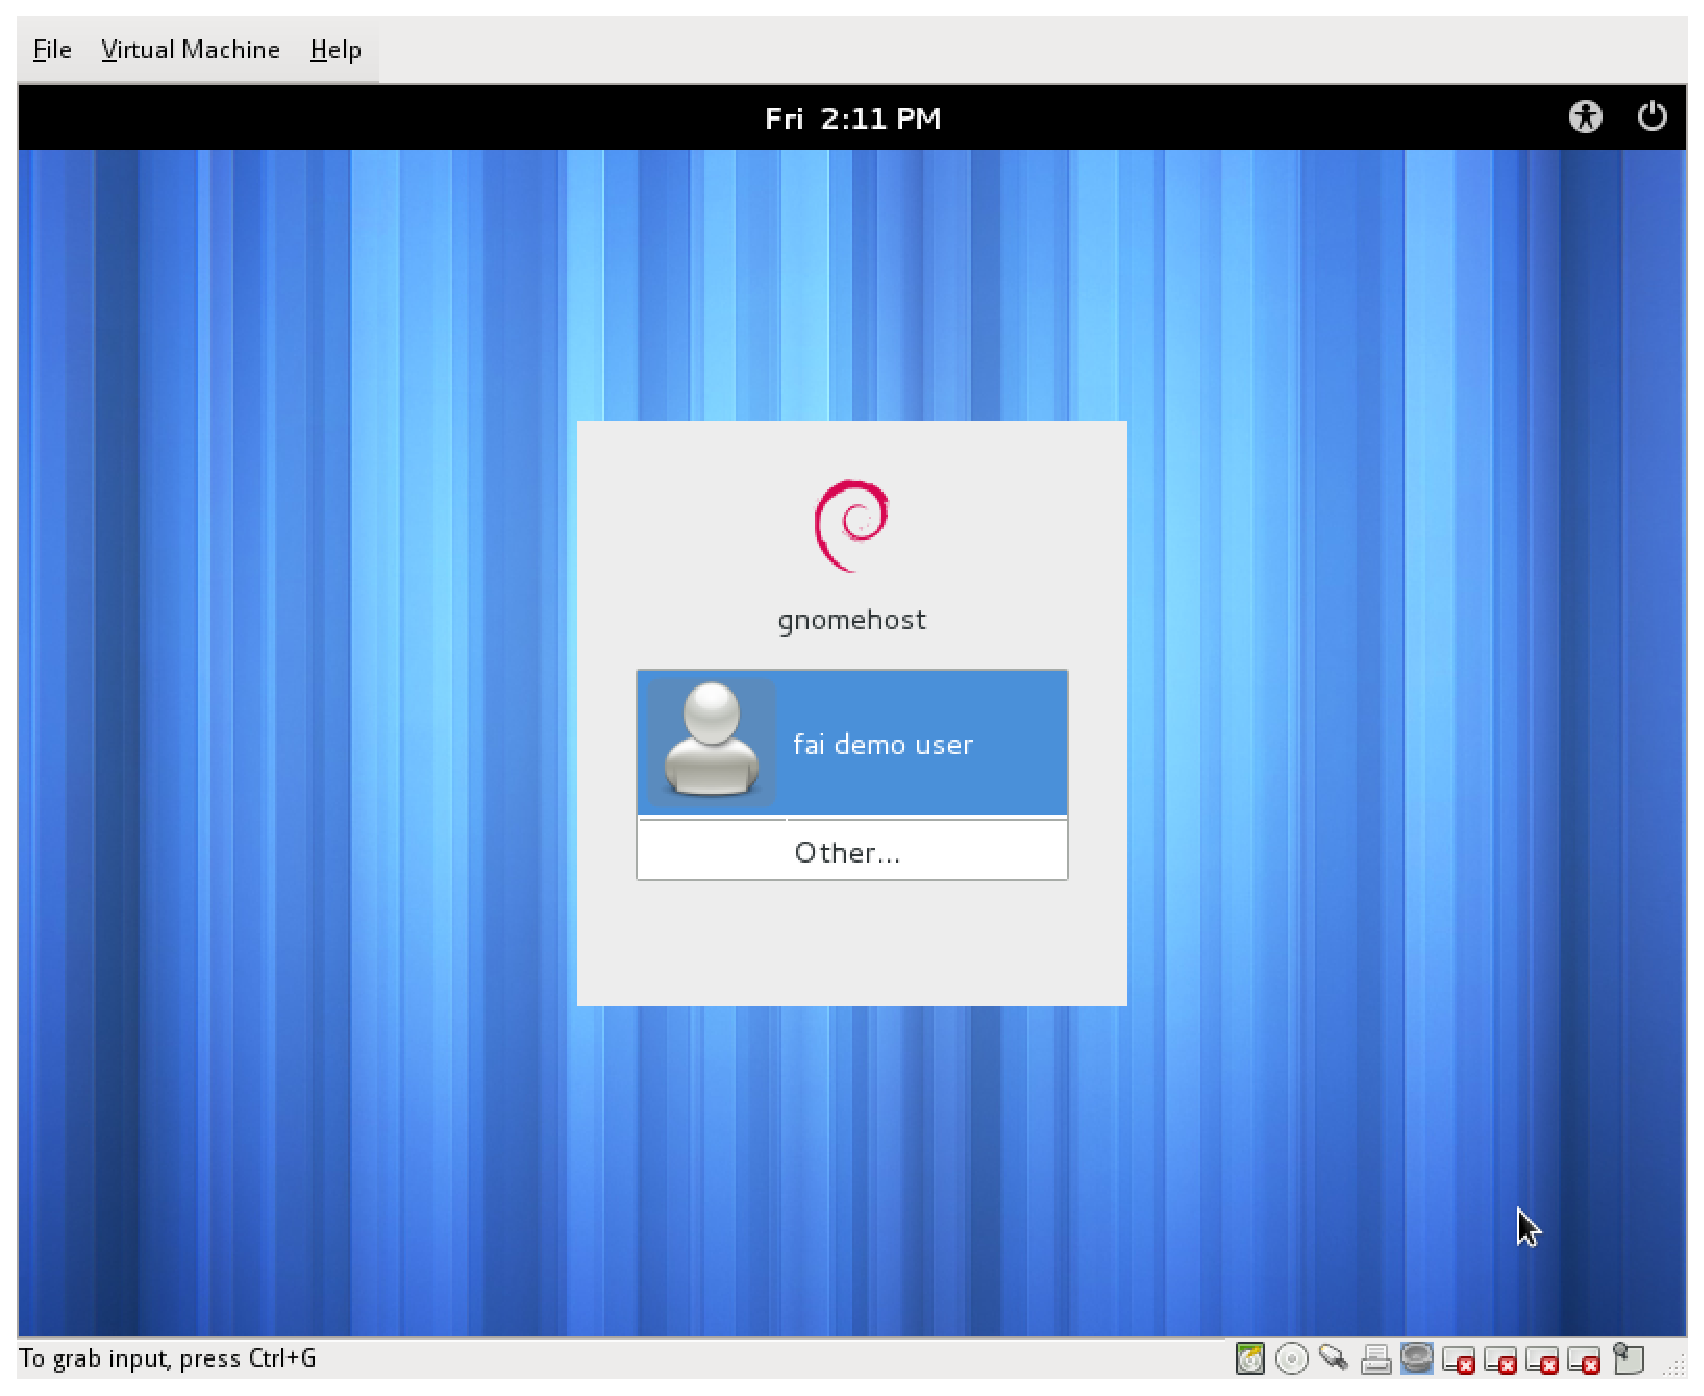
\includegraphics[width=0.45\textwidth]{./images/f-4.eps}
	      \label{fig:f-4}
	    }
            \hfill
  \subbottom[IP address in Gnome terminal]
	    {
	      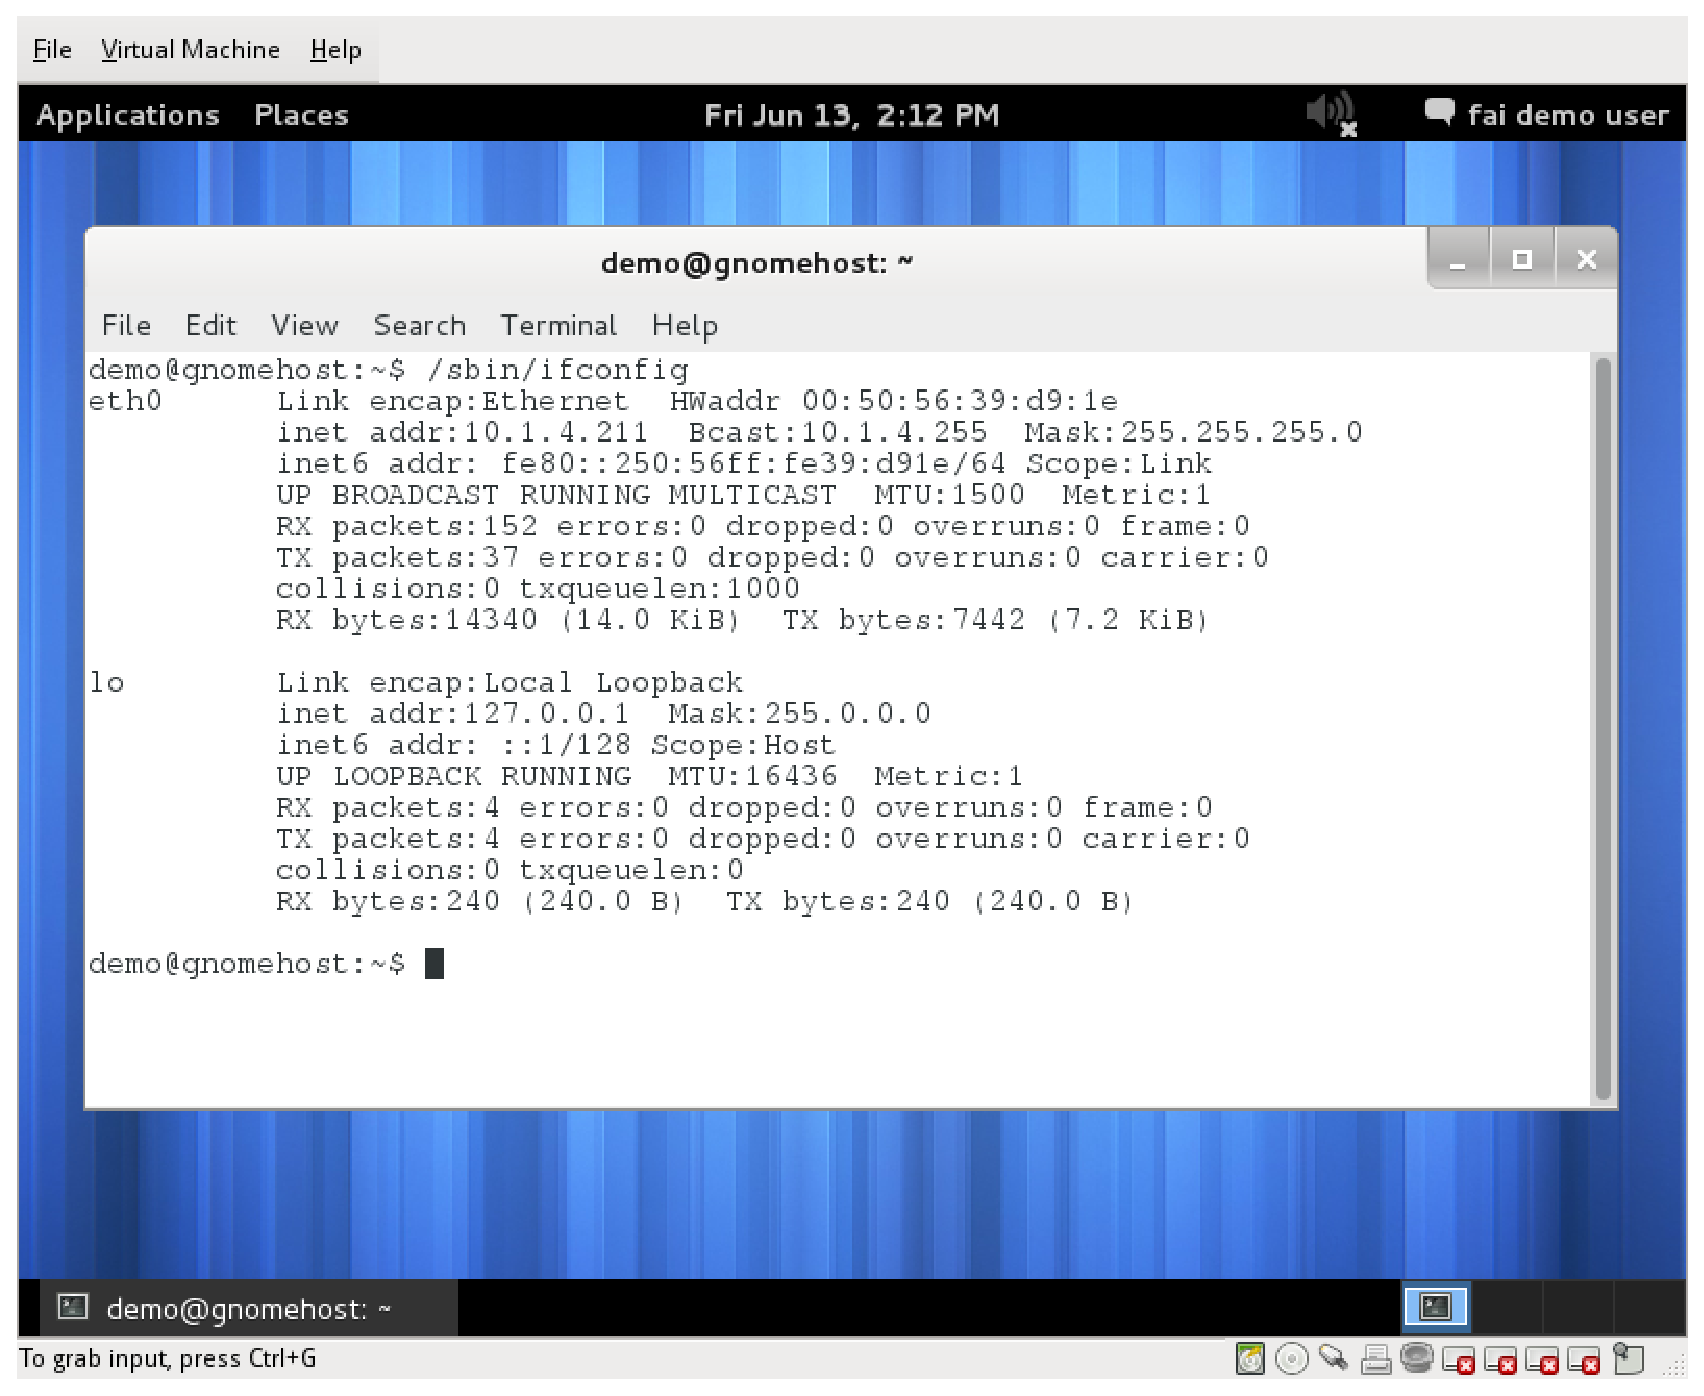
\includegraphics[width=0.45\textwidth]{./images/f-5.eps}
	      \label{fig:f-5}
	    }
  \caption
      {
        FAI Installation screehshots and the installed Debian Linux
      }
 \label{fig:gnomehost}
\end{figure}



%\clearpage

\bibliographystyle{unsrtnat}

\bibliography{./refs}




\end{document}
